\section{Démarche}\label{sec:demarche}

\subsection{Matériel}\label{subsec:materiel}
Pour pouvoir réaliser l’expérience nous avons besoin de :
\begin{itemize}
    \item Glycérine
    \item Un cylindre gradué (privilégié une longueur plutôt qu'un gros volume)
    \item De 2 ou 3 billes ayant des rayons différents (en acier dans notre cas)
    \item Un aimant (pour récuperer les billes)
    \item Un entonnoir (pour ne pas verser à côté la glycérine)
    \item Un chronomètre
    \item Un marqueur
\end{itemize}

\subsection{Marche à suivre}\label{subsec:marche-a-suivre}
\begin{enumerate}
    \item Remplir le cylindre gradué de glycérine a l’aide de l’entonnoir et récupérer tous les autres accessoires nécessaires à l’expérience dans le laboratoire (voir matériel).
    \item Tracer deux marques sur le cylindre gradué en utilisant le marqueur.
    Il est conseillé de les tracer à une certaine distance (x = 8.5 [cm] dans notre cas) car le plus écartées sont les marques, le plus les résultats seront fiables.
    Il serait aussi envisageable de ne pas mettre de traces trop hautes non plus, pour ne pas commencer le chronomètre pendant que la bille subit une accélération.
    \item Lâcher la bille au dessus du liquide à l’aide de ses doigts.
    \item Commencer le chronomètre lorsque la bille atteint la première marque puis l’arrêter une fois traversée la deuxième marque.
    \item Prendre note du temps pris pour que la bille fasse x centimètres dans le fluide à vitesse constante.
    \item Récupérer la bille en utilisant l’aimant (le mettre contre le cylindre, et monter jusqu’en haut gentiment lorsque la bille se fait attirer).
    \item Répéter l’expérience plusieurs fois afin d’en faire une moyenne, puis changer le rayon de la bille.
\end{enumerate}

\subsection{Schéma de l'expérience}\label{subsec:schema}
\begin{figure}[H]
    \centering
    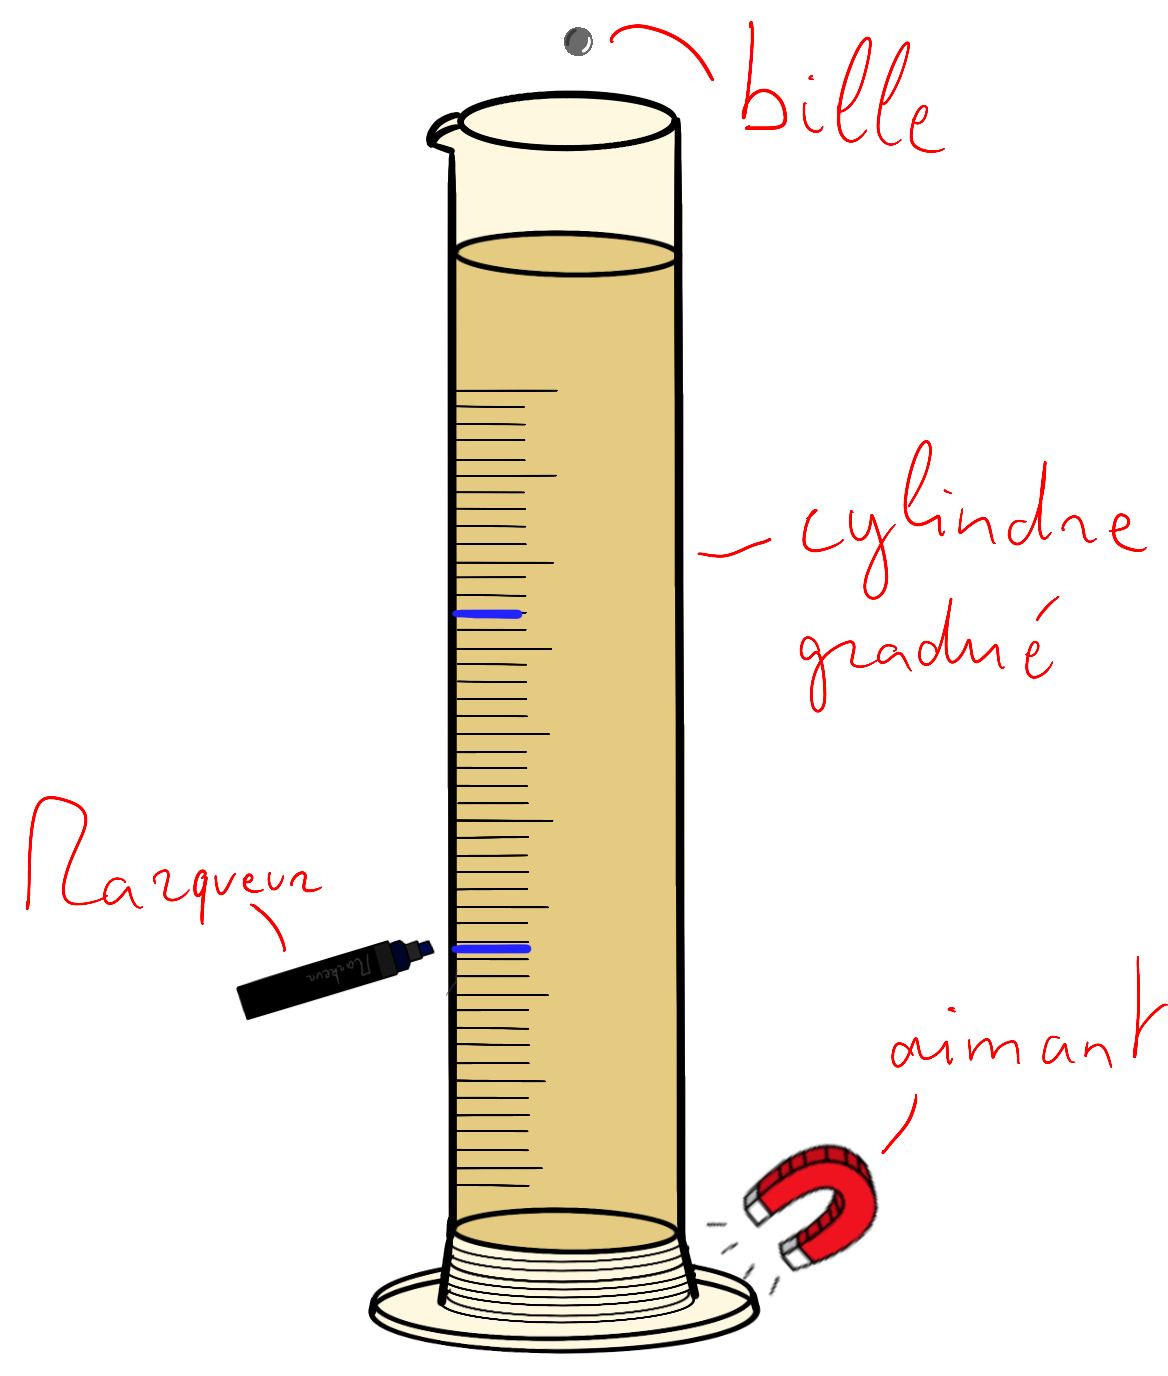
\includegraphics[scale=0.45]{graph/schema-exp}
    \caption{Schéma de l'expérience}
    \label{fig:schema-exp}
\end{figure}